%%%%%%%%%%%%%%%%%%%%%%%%%%%%%%%%%%%%%%%%%%%%%%%%%%%
%% P3: Phenomenology of Particle Physics                         
%%
%% Author:  André Rubbia                   		 
%%
%% Figure 3.4 The concept of the cyclotron. 
%%
%% This work is licensed under the Creative Commons Attribution 4.0 International License. 
%% To view a copy of this license, visit http://creativecommons.org/licenses/by/4.0/ or 
%% send a letter to Creative Commons, PO Box 1866, Mountain View, CA 94042, USA.
%%
%%%%%%%%%%%%%%%%%%%%%%%%%%%%%%%%%%%%%%%%%%%%%%%%%%%

\documentclass[a4paper,10pt]{article}

\usepackage[T1]{fontenc}
\usepackage[utf8]{inputenc}
\usepackage{lmodern}
\usepackage[labelfont=bf]{caption}
\usepackage{upgreek}

\usepackage{tikz}
\usepackage{pgfplots}
\pgfplotsset{compat=1.17}
\usepgfplotslibrary{ternary}
\usepgfplotslibrary{fillbetween}
\usepgfplotslibrary{external}

\def\d{\mathrm{d}}

\begin{document}

%%%%%%%%%%%%%%%   FIGURE  %%%%%%%%%%%%%%%%%%%%%%%%%%%%%%
\begin{figure}[htb]
\begin{center}
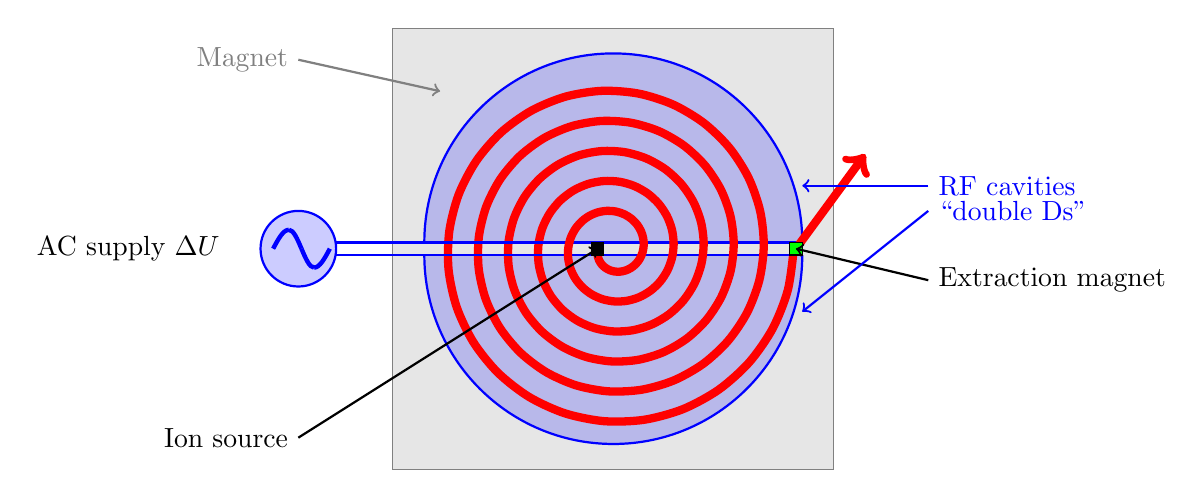
\begin{tikzpicture}[scale=0.8]
     \draw[gray,fill,fill opacity=0.2] (-3.5,-3.5) rectangle (3.5,3.5);
    \draw[blue,thick,fill opacity=0.2,fill=blue] (3,0.1) arc[radius=3, start angle=0, end angle=180];
    \draw[blue,thick,fill opacity=0.2,fill=blue] (3,-0.1) arc[radius=3, start angle=0, end angle=-180];
    \draw[blue,thick] (-3,0.1) -- (3,0.1);
    \draw[blue,thick] (-3,-0.1) -- (3,-0.1);
    \draw [red, line width=3pt, domain=3.14:37.7,variable=\t,smooth,samples=150]
        plot ({\t r}: {0.076*\t});
     \draw[red, line width=3pt,->] (2.9,0) -- (4,1.5);
     \draw[fill=green] (2.8,-0.1) rectangle +(0.2,0.2);
     \draw[fill=black] (-0.35,-0.1) rectangle +(0.2,0.2);
     \draw[thick,gray,->] (-5,3) node[left] {Magnet} -- (-2.75,2.5);
     \draw[thick,->] (-5,-3) node[left] {Ion source} -- (-0.25,0);
     \draw[thick,black,->] (5,-0.5) node[right] {Extraction magnet} -- (2.9,0);
     \draw[thick,blue,->] (5,1) node[right] {RF cavities} -- (3,1);
     \draw[thick,blue,->] (5,0.6) node[right] {``double Ds''} -- (3,-1);
     \draw[blue,thick,fill opacity=0.2,fill=blue] (-5,0) circle (0.6);
     \draw[blue,thick] (-4.4,-0.1) -- (-1.12,-0.1);
     \draw[blue,thick] (-4.4,0.1) -- (-1.12,0.1);
     \node at (-7.7,0) {AC supply $\Delta U$};
     \draw[ultra thick, blue] (-5.4,0) sin (-5.15,0.3);
     \draw[ultra thick, blue] (-5.15,0.3) cos (-4.95,0);
     \draw[ultra thick, blue] (-4.95,0) sin (-4.75,-0.3);
     \draw[ultra thick, blue] (-4.75,-0.3) cos (-4.5,0);
\end{tikzpicture}
\caption{The concept of the cyclotron. The spiralling trajectory of a particle is shown as a thick line.
The particle is eventually extracted with a magnet at the outer radius of the cyclotron.}
\end{center}
\end{figure}
%

\end{document}
